\documentclass[11pt,justified]{beamer}
\mode<presentation>
\let\Tiny=\tiny
\usetheme{CambridgeUS}
\usefonttheme{professionalfonts}
\usepackage[brazil]{babel}
\usepackage[utf8]{inputenc}
\usepackage{amsfonts}
\usepackage{amssymb}
\usepackage{amsmath}
\usepackage{listings}

\lstset{basicstyle=\scriptsize,language=Java, showstringspaces=false}

\newcommand\blfootnote[1]{%
  \begingroup
  \renewcommand\thefootnote{}\footnote{#1}%
  \addtocounter{footnote}{-1}%
  \endgroup
}

\title{Introdução à Programação Concorrente em Java}
\author{}
\date{}

\begin{document}

\begin{frame}[plain]
    \titlepage
\end{frame}

\section{Sistemas multitarefas}

\begin{frame}{Sistemas multitarefas}
    \begin{itemize}
        \item Sabe-se que a CPU executa apenas um programa por vez.
        \item A princípio, se esta regra for seguida de maneira estrita, é impossível utilizar os computadores do modo como é feito hoje, com diversos programas sendo executados ao mesmo tempo.
        \item Torna-se necessário, então, a criação de sistemas multitarefas.
    \end{itemize}
\end{frame}

\begin{frame}{Sistemas multitarefas}
    \begin{itemize}
        \item Um sistema multitarefas executa diversos programas de maneira alternada.
        \item A troca de programa na CPU (troca de contexto) é realizada tão rapidamente que os programas parecem rodas em paralelo (pseudoparalelismo).
    \end{itemize}
\end{frame}

\begin{frame}{Sistemas multitarefas}
    \begin{itemize}
        \item Mesmo em sistemas com diversas CPUs, o número de programas tende a ser maior que o número de CPUs.
        \item Então, a troca de contexto ainda é presente em ambientes multiprocessados.
    \end{itemize}
\end{frame}

\section{Processos e \textit{threads}}

\begin{frame}{Processos}
    \begin{itemize}
        \item A unidade de armazenamento (estrutura de dados) de um programa é o processo.
        \item O processo armazena todos os dados e instruções da execução do programa.
    \end{itemize}
\end{frame}

\begin{frame}{Processos}
    De maneira simplória, os processos podem realizar dois tipos de instruções fundamentais:
    \begin{itemize}
        \item processamento de dados;
        \item entrada e saída de dados;
    \end{itemize}
\end{frame}

\begin{frame}{Processos}
    \begin{itemize}
        \item A entrada e saída de dados é muito custosa, pois depende de dispositivos muito lentos em relação à CPU.
        \item De modo geral, a espera pelas operações de entrada e saída de dados torna o programa inerte durante este período.
        \item Para evitar o desperdício de recursos, pode-se ter um processo dividido em subprocessos, cada um com seu espaço de armazenamento.
    \end{itemize}
\end{frame}

\begin{frame}{Subprocessos}
    \begin{itemize}
        \item O problema dos subprocessos está na carestia de tempo de processamento e memória para criá-los.
        \item Além disso, a comunicação entre processos exige estruturas de dados e técnicas específicas.
    \end{itemize}
\end{frame}

\begin{frame}{\textit{Threads}}
    \begin{itemize}
        \item Para mitigar alguns problemas da criação de subprocessos, tem-se o conceito de \textit{threads}.
        \item Grosso modo, uma \textit{thread} é um programa que compartilha o espaço de endereçamento com outras \textit{threads}.
    \end{itemize}
\end{frame}

\begin{frame}{\textit{Threads}}
    \begin{itemize}
        \item A comunicação entre \textit{threads} é mais simples que entre processos, pois as \textit{threads} dentro de um mesmo processo compartilham o mesmo espaço de armazenamento.
        \item A criação de \textit{threads} também é bastante mais rápida que a de subprocessos.
        \item Apesar disto, o uso de \textit{threads} não elimina completamente o \textit{overhead}, as condições de corrida e de impasse e possíveis situações de inconsistência.
    \end{itemize}
\end{frame}

\section{\textit{Threads} de SO e \textit{threads} Java}

\begin{frame}{\textit{Threads} de SO}
    Para os sistemas operacionais modernos há, comumente, dois tipos de \textit{threads}:
    \begin{itemize}
        \item \textit{thread} de sistema;
        \item \textit{thread} de usuário.
    \end{itemize}
\end{frame}

\begin{frame}{\textit{Threads} Java}
    \begin{itemize}
        \item As \textit{threads} em Java são todas \textit{threads} de usuário.
        \item Apesar de criadas pela JVM, as \textit{threads} são criadas como nativas do SO através do uso de bibliotecas.
        \item A implementação e o mapeamento destas \textit{threads} dependerá da implementação da JVM.
    \end{itemize}
\end{frame}


\begin{frame}{\textit{Threads} Java}
    Internamente, a JVM possui dois tipos de \textit{threads}:
    \begin{itemize}
        \item \textit{threads} de usuário;
        \item \textit{threads daemon}.
    \end{itemize}
\end{frame}

\begin{frame}{\textit{Threads} Java}
    \begin{itemize}
        \item Para a JVM, o método \textit{main} é uma \textit{thread} de usuário chamada \textit{main}.
        \item Mesmo que \textit{thread main} seja completada, enquanto existirem \textit{thread} de usuário ativas, o programação não será encerrado.
        \item Isto não é válido para \textit{threads daemon}.
    \end{itemize}
\end{frame}

\begin{frame}{\textit{Threads} Java}
    \begin{itemize}
        \item Se todas as \textit{threads} de usuário forem encerradas, a JVM pode encerrar arbitrariamente as \textit{threads daemon}.
        \item Por isso, \textit{threads daemon} devem executar tarefas de suporte em \textit{background}, como \textit{garbage collection}.
    \end{itemize}
\end{frame}

\section{Criação de \textit{threads} em Java}

\begin{frame}{Criação de \textit{Threads} em Java}
    As \textit{threads}, em Java, podem ser criadas através de dois modos:
    \begin{itemize}
        \item herança da classe \textit{Thread};
        \item implementação da \textit{interface Runnable}.
    \end{itemize}
\end{frame}

\begin{frame}[fragile]{Herança da classe \textit{Thread}}
    Exemplo de criação de \textit{thread} em Java pela herança da classe \textit{Thread}:
    \begin{lstlisting}
public class MyThread extends Thread {
    public void run() {
        System.out.println("====== Starting " + 
            this.getName() + " thread ======");
        for (int i = 0; i < 5; i++) {
            System.out.println("The thread " + 
                this.getName() + " prints " + i);
        }
        System.out.println("====== Finishing " + 
            this.getName() + " thread ======");
    }
}
    \end{lstlisting}
\end{frame}

\begin{frame}[fragile]{Herança da classe \textit{Thread}}
    Exemplo de criação de \textit{thread} em Java pela herança da classe \textit{Thread} (continuação):
    \begin{lstlisting}
public static void main(String[] args) {
    System.out.println("====== Starting main thread ======");
    MyThread t1 = new MyThread();
    MyThread t2 = new MyThread();
    
    t1.start();
    t2.start();
    for (int i = 0; i < 5; i++) {
        System.out.println("Main thread prints " + i);
    }
    System.out.println("====== Finishing main thread ======");
}
    \end{lstlisting}
\end{frame}

\begin{frame}{Herança da classe \textit{Thread}}
    \begin{itemize}
        \item A saída do programa pode variar porque, neste caso, não há como especificar a ordem de execução das \textit{threads}.
        \item O método \textit{start} é reponsável por iniciar a \textit{thread}.
        \item Toda \textit{thread} em Java deve sobrescrever o método \textit{run}.
    \end{itemize}
\end{frame}

\begin{frame}[fragile]{Implementação da \textit{interface Runnable}}
    Outro modo de criar uma \textit{thread} em Java é implementar a \textit{interface Runnable}:
    \begin{lstlisting}
public class MyRunnable implements Runnable {
    public void run() {
        System.out.println("====== Starting runnable ======");
        for (int i = 0; i < 5; i++) {
            System.out.println("A runnable prints " + i);
        }
        System.out.println("====== Finishing runnable ======");
    }
}
    \end{lstlisting}
\end{frame}

\begin{frame}[fragile]{Implementação da \textit{interface Runnable}}
    O método \textit{main} permanece quase idêntico:
    \begin{lstlisting}
public static void main(String[] args) {
    System.out.println("====== Starting main thread ======");
    Thread t1 = new Thread(new MyRunnable());
    Thread t2 = new Thread(new MyRunnable());
    
    t1.start();
    t2.start();
    for (int i = 0; i < 5; i++) {
        System.out.println("Main thread prints " + i);
    }
    System.out.println("====== Finishing main thread ======");
}
    \end{lstlisting}
\end{frame}

\begin{frame}{Implementação da \textit{interface Runnable}}
    \begin{itemize}
        \item Note que no exemplo, são criadas dois objetos \textit{Thread}.
        \item No construtor de cada um é passado um objeto que implementa a \textit{interface Runnable}.
        \item A classe \textit{Thread} tem diversos construtores que podem ser utilizados para dar mais flexibilidade ao programador.
    \end{itemize}
\end{frame}

\begin{frame}{Implementação da \textit{interface Runnable}}
    \begin{itemize}
        \item Um ponto interessante é que a implementação de \textit{Runnable} exige também sobrescrever \textit{run}.
        \item Mais do que isso, \textit{Thread} também implementa \textit{Runnable}.
        \item Por isso possui um método \textit{run}.
    \end{itemize}
\end{frame}

\begin{frame}{Criação de \textit{threads} em Java}
    \begin{itemize}
        \item Implementar a \textit{interface Runnable} é preferencial em relação à herdar a classe \textit{Thread}.
        \item Java não aceita herança múltipla, mas aceita a implementação de mais de uma \textit{interface}.
        \item Assim, implementar \textit{Runnable} torna-se mais vantajoso.
        \item Além disso, implementar \textit{interfaces} é quase sempre melhor do ponto de vista de coesão/acoplamento entre as classes.
        \item Só se deve herdar de \textit{Thread} se for necessário sobrescrever outros métodos de \textit{Thread} além de \textit{run}.
    \end{itemize}
\end{frame}

\begin{frame}{Estados das \textit{threads} em Java}
    \begin{figure}[ht]
        \centering
        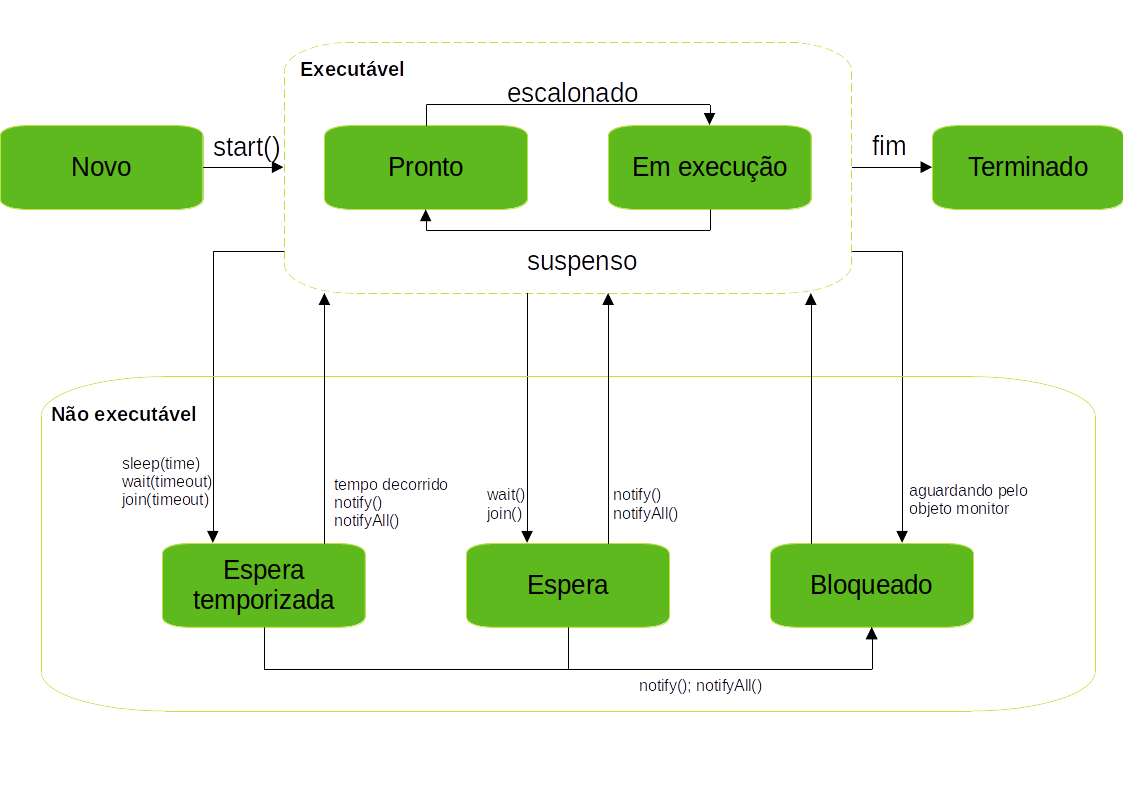
\includegraphics[height=7.6cm, width=10cm]{figures/thread_ciclo_de_vida.png}
    \end{figure}
\end{frame}

\begin{frame}{Método \textit{sleep}}
    \begin{itemize}
        \item Um modo de parar temporariamente uma \textit{thread} é o método \textit{sleep} (da classe \textit{Thread}).
        \item Ao executar este método, a \textit{thread} passa para um estado não-executável (espera temporizada).
        \item A \textit{thread} volta ao estado de pronto assim que o tempo é decorrido ou caso o método \textit{sleep} levante uma \textit{InterruptionException}.
    \end{itemize}
\end{frame}

\begin{frame}[fragile]{Método \textit{sleep}}
    \begin{lstlisting}
public class SleepingThread implements Runnable {
    public void run() {
        for (int i = 0; i < 5; i++) {
            try {
                    System.out.println("A runnable prints " + i);
                    Thread.sleep(4000);
            } catch (InterruptedException e) {
                e.printStackTrace();
            }
        }
    }
}
    \end{lstlisting}
\end{frame}

\begin{frame}[fragile]{Método \textit{sleep}}
    \begin{lstlisting}
public static void main(String[] args) {
    Thread t1 = new Thread(new SleepingThread());
    t1.start();
}
    \end{lstlisting}
\end{frame}

\begin{frame}[fragile]{\textit{Threads daemon}}
    Agora, com o método \textit{sleep}, pode-se exemplificar a diferença entre \textit{threads} de usuário e \textit{threads daemon}:
    \begin{lstlisting}
        public class UserOrDaemonThread extends Thread {
            public int sleepingTime = 0;
            public void run() {
                for (int i = 0; i < 5; i++) {
                    try {
                        Thread.sleep(this.sleepingTime);
                        System.out.println("The thread " + 
                            this.getName() + " prints " + i);
                    } catch (InterruptedException e) {
                        e.printStackTrace();
                    }
                }
            }
        }
    \end{lstlisting}
\end{frame}

\begin{frame}[fragile]{\textit{Threads daemon}}
    \begin{lstlisting}
public static void main(String[] args) {
    UserOrDaemonThread t1 = new UserOrDaemonThread();
    UserOrDaemonThread t2 = new UserOrDaemonThread();
    t1.sleepingTime = 1000;
    t2.sleepingTime = 2000;
    t2.setDaemon(true);
    t1.start();
    t2.start();
}
    \end{lstlisting}

    Na saída do programa, será possível observar que a \textit{thread} \textbf{t2} não é executada até o fim.
\end{frame}

\begin{frame}{Problema de produtor/consumidor}
    \begin{itemize}
        \item Um problema clássico da computação concorrente é o problema de produtor/consumidor.
        \item Neste problema, há um ou mais produtores que inserem o "produto" em um \textit{buffer} e um ou mais consumidores que consomem o conteúdo deste mesmo \textit{buffer}.
    \end{itemize}
\end{frame}

\begin{frame}{Problema de produtor/consumidor}
    \begin{itemize}
        \item O desafio é garantir que produtores e consumidores trabalhem de maneira sincronizada.
        \item O \textit{buffer} só pode ser acessado por um agente por vez.
        \item O consumidor só pode consumir se existir algum produto ainda não consumido no \textit{buffer}.
    \end{itemize}
\end{frame}

\begin{frame}{Problema de produtor/consumidor}
    \begin{itemize}
        \item Morelli e Walde apresentam um exemplo para ilustrar o problema de produtor/consumidor na vida real.Artuss
        \item Tenha-se uma padaria onde os clientes pegam uma senha e são atendidos em ordem.
        \item Esta situação, assim como várias onde há fila, pode ser vista como um problema de produtor/consumidor.
        \item O cliente é o produtor (pois pede uma senha).
        \item O atendente é o consumidor (pois consome uma senha gerada).
        \item A máquina de senha é o \textit{buffer}.
    \end{itemize}
\end{frame}

\begin{frame}{Problema de produtor/consumidor}
    \begin{itemize}
        \item A máquina de senha deve manter a contagem e não pode pular números e/ou clientes.
        \item Dois clientes não podem ter o mesmo número.
        \item O atendente não pode atender um cliente inexistente.
    \end{itemize}
\end{frame}

\begin{frame}{Problema de produtor/consumidor}
    Para resolver este problema, deve-se decompo-lo em partes menores:
    \begin{itemize}
        \item um objeto para a máquina de senha;
        \item uma classe representando o(s) atendente(s);
        \item uma classe representando o(s) cliente(s);
        \item o cliente pede um número à máquina;
        \item o atendente atende o próximo número da fila;
        \item uma classe para padaria que terá o \textit{main} e criará as \textit{threads}.
    \end{itemize}
\end{frame}


\begin{frame}[fragile]{Máquina de senha (classe \textit{TakeANumber})}
    \begin{lstlisting}
public class TakeANumber {
    private int next = 0;
    private int serving = 0;
    public int nextNumber() {
        next = next + 1; return next;
    }
    public int nextCustomer() {
        ++serving; return serving;
    }
    public boolean thereIsCustomerWaiting() {
        return next > serving;
    }
}
    \end{lstlisting}\blfootnote{Adaptado de Morelli e Walde.}
    \begin{itemize}
        \item \textit{nextNumber} e \textit{nextCustomer} são chamados por clientes e atendentes respectivamente.
        \item \textit{thereIsCustomerWaiting} é para garantir que não serão atendidas senhas inexistentes.
    \end{itemize}
\end{frame}

\begin{frame}[fragile]{Cliente (classe \textit{Customer})}
    A classe \textit{Customer} é bastante trivial.
    \begin{lstlisting}
public class Customer extends Thread {
    private static int number = 10000;
    private int id;
    private TakeANumber takeANumber;
  
    public Customer( TakeANumber gadget ) {
      id = ++number; takeANumber = gadget;
    }
    public void run() {
      try {
        sleep( (int)(Math.random() * 1000 ) );
        System.out.println("Customer " + id +
         " takes ticket " + takeANumber.nextNumber());
      } catch (InterruptedException e) {
        System.out.println("Exception " + e.getMessage());
      }
    }
}
    \end{lstlisting}\blfootnote{Adaptado de Morelli e Walde.}
\end{frame}

\begin{frame}[fragile]{Atendente (classe \textit{Clerk})}
    A classe \textit{Clerk} é também bastante trivial.
    \begin{lstlisting}
public class Clerk extends Thread {
    private TakeANumber takeANumber;

    public Clerk(TakeANumber gadget) {
        takeANumber = gadget;
    }
    public void run() {
        while (true) {
            try {
                sleep((int)(Math.random() * 50));
                if (takeANumber.thereIsCustomerWaiting())
                    System.out.println("Clerk serving ticket " +
                        takeANumber.nextCustomer());
            } catch (InterruptedException e) {
                System.out.println("Exception " + e.getMessage() );
            }
        }
    }
}
    \end{lstlisting}\blfootnote{Adaptado de Morelli e Walde.}
\end{frame}

\begin{frame}[fragile]{Padaria (classe \textit{Bakery})}
    \begin{lstlisting}
public class Bakery {
    public static void main(String args[]) {
        System.out.println("Starting clerk and customer threads");
        TakeANumber numberGadget = new TakeANumber();
        Clerk clerk = new Clerk(numberGadget);
        clerk.start();
        for (int k = 0; k < 5; k++) {
            Customer customer = new Customer(numberGadget);
            customer.start();
        }
    }
}
    \end{lstlisting}\blfootnote{Adaptado de Morelli e Walde.}
\end{frame}

\begin{frame}{Problema de produtor/consumidor}
    \begin{itemize}
        \item A solução apresentada pode, a princípio, parecer correta.
        \item Entretanto, o código não é seguro e apresentará problemas quando houver situações de concorrência.
    \end{itemize}
\end{frame}

\begin{frame}[fragile]{Sincronização de \textit{threads}}
    Tenha-se o código do método \textit{nextNumber}:
    \begin{lstlisting}
public int nextNumber() {
    next = next + 1;
    return next;
}
    \end{lstlisting}\blfootnote{Adaptado de Morelli e Walde.}
    \begin{itemize}
        \item Nada garante que a \textit{thread} executando este código não será retirada da CPU entre a primeira e segunda instrução.
        \item Caso isso ocorra, outra \textit{thread} poderá também chamar \textit{nextNumber}, o que poderá causar que dois clientes peguem a mesma senha e que algumas senhas sejam "puladas".
    \end{itemize}
\end{frame}

\begin{frame}[fragile]{Sincronização de \textit{threads}}
    Para simular este problema, basta chamar o método \textit{sleep} entre as duas instruções:
    \begin{lstlisting}
public int nextNumber() {
    next = next + 1;
    try {
        Thread.sleep(100);
    } catch (InterruptedException e) {}
    return next;
}
    \end{lstlisting}
    Ao executar o código, será possível notar que mais de um cliente terá a mesma senha.\blfootnote{Algumas vezes a mensagem do atendente atendendo antes da mensagem do cliente pegar a senha pode aparecer, mas isso se dá porque o foi chamado o métodos \textit{sleep}, atrasando a \textit{thread} do cliente.}
\end{frame}

\begin{frame}{Região crítica}
    \begin{itemize}
        \item As duas linhas originais de \textit{nextNumber} formam a chamada região crítica.
        \item A região crítica é uma região do código que deve ser executada de maneira atômica, para evitar possíveis inconsistências em condições de concorrência.
    \end{itemize}
\end{frame}

\begin{frame}{Bloco \textit{synchronized}}
    \begin{itemize}
        \item Java permite que um bloco de código seja declarado como uma região crítica.
        \item Para isto, usa-se a palavra-chave \textit{synchronized}, além de um objeto que servirá como monitor.
        \item Este monitor pode ser todo e qualquer objeto.
        \item Ao entrar em uma região crítica, a \textit{thread} executora deve conseguir o \textit{lock} deste objeto.
        \item Se outra \textit{thread} tentar entrar na mesma região crítica ou que tenha o mesmo objeto monitor, esta deverá aguardar até que a \textit{thread} que possui o \textit{lock} o largue.
    \end{itemize}
\end{frame}

\begin{frame}[fragile]{Bloco \textit{synchronized}}
    Além de modificar \textit{nextNumber}, adicionou-se um atributo \textit{o} do tipo \textit{Object}:
    \begin{lstlisting}
private Object o = new Object();
public int nextNumber() {
    synchronized (o) {
        next = next + 1;
        try {
            Thread.sleep(100);
        } catch (InterruptedException e) {}
        return next;
    }
}
    \end{lstlisting}\footnote{O mesmo se aplica ao método \textit{nextCustomer} caso haja mais de um atendente.}
\end{frame}

\begin{frame}{Método \textit{synchronized}}
    \begin{itemize}
        \item Algumas vezes, teremos a necessidade que o método inteiro seja região crítica.
        \item Para isto, Java permite que um método seja declarado como \textit{synchronized}.
    \end{itemize}
\end{frame}

\begin{frame}[fragile]{Método \textit{synchronized}}
    Retira-se o atributo \textit{o} e modifica-se \textit{nextNumber}:
    \begin{lstlisting}
public synchronized int nextNumber() {
    next = next + 1;
    try {
        Thread.sleep(100);
    } catch (InterruptedException e) {}
    return next;
}
    \end{lstlisting}\footnote{Para garantir a segurança do código como um todo, é interessante declarar como sincronizados os outros dois métodos de \textit{TakeANumber}.}
\end{frame}

\begin{frame}[fragile]{Método \textit{synchronized}}
    \begin{itemize}
        \item Em métodos \textit{synchronized} o monitor é o próprio objeto.
        \item Neste caso, a instância de \textit{TakeANumber}.
        \item Seria como:
    \end{itemize}
    \begin{lstlisting}
public int nextNumber() {
    synchronized(this) {
        next = next + 1;
        try {
            Thread.sleep(100);
        } catch (InterruptedException e) {}
        return next;
    }
}
    \end{lstlisting}
\end{frame}

\begin{frame}{Problema da espera-ocupada}
    \begin{itemize}
        \item Um problema do exemplo atual é que a \textit{thread Clerk}, por estar executando em um laço infinito, continua tomando tempo da CPU mesmo quando não há clientes com senhas.
        \item A esta situação é dado nome de espera-ocupada.
        \item Para evitar isso, Java possui um mecanismo de espera/notificação, que coloca a \textit{thread} em estado de espera, evitando que entre na CPU.
    \end{itemize}
\end{frame}

\begin{frame}[fragile]{Mecanismo de espera/notificação}
    \begin{lstlisting}
public synchronized int nextCustomer() {
    try {
      while (next <= serving)
        wait();
    } catch(InterruptedException e) {
    } finally {
      ++serving;
      System.out.println("Clerk serving ticket " + serving);
      return serving;
    }
  }
\end{lstlisting}
    Quando não houver clientes desassistidos (next $<=$ serving), a \textit{thread} que invocar \textit{nextCustomer} ficará aguardando (método \textit{wait}).\blfootnote{Não há mais a necessidade de \textit{thereIsCustomerWaiting}.}
\end{frame}

\begin{frame}{Mecanismo de espera/notificação}
    \begin{itemize}
        \item Caso não seja passado um tempo limite para \textit{wait}, a \textit{thread} ficará esperando indefinidamente.
        \item Por isso, é preciso que outra \textit{thread} notifique a \textit{thread} que está aguardando.
        \item No caso aqui descrito, o método \textit{nextNumber} será o responsável por notificar as \textit{thread} aguardando.
    \end{itemize}
\end{frame}

\begin{frame}[fragile]{Mecanismo de espera/notificação}
    \begin{lstlisting}
public synchronized int nextNumber(int custId) {
    next = next + 1;
    System.out.println("Customer " + custId + 
        " takes ticket " + next);
    notify();
    return next;
}
    \end{lstlisting}
\end{frame}

\begin{frame}{\textit{notify} e \textit{notifyAll}}
    \begin{itemize}
        \item O método \textit{notify} notifica a \textit{thread} mais a frente na fila de \textit{threads} em estado de aguardo.
        \item Já o método \textit{notifyAll} notifica todas as \textit{threads} que estão aguardando.
        \item Por isso, o método \textit{wait} é chamado dentro de um laço, pois, caso contrário, todas as \textit{threads Clerk} executariam os códigos da sua cláusula \textit{finally}.
    \end{itemize}
\end{frame}


\begin{frame}[fragile]{classe \textit{TakeANumber} - versão final}
    \begin{lstlisting}
public class TakeANumber {
    private int next = 0; private int serving = 0;
    public synchronized int nextNumber(int custId) {
        next = next + 1;
        System.out.println("Customer:" + custId + 
            " takes ticket " + this.next);
        notify();
        return next;
    } 
    public synchronized int nextCustomer() {
        try {
            while (next <= serving) {
                System.out.println("Clerk waiting ");
                wait();
            }
        } catch (InterruptedException e) {
        } finally {
            ++serving;
            System.out.println("Clerk serving ticket " + serving);
            return serving;
        }
    }
}
    \end{lstlisting}\blfootnote{Adaptado de Morelli e Walde.}
\end{frame}

\begin{frame}[fragile]{classe \textit{Clerk} - versão final}
    \begin{lstlisting}
public class Clerk extends Thread {
    private TakeANumber takeANumber;
    public Clerk(TakeANumber gadget) {
        this.takeANumber = gadget;
    }
    public void run() {
        while (true) {
            try {
                sleep((int) (Math.random() * 50));
                takeANumber.nextCustomer();
            } catch (InterruptedException e) {}
        }
    }   
}
    \end{lstlisting}\blfootnote{Adaptado de Morelli e Walde.}
\end{frame}

\begin{frame}[fragile]{classe \textit{Customer} - versão final}
    \begin{lstlisting}
public class Customer extends Thread {
    private static int number = 10000;
    private int id;
    private TakeANumber takeANumber;
    public Customer(TakeANumber gadget) {
        this.id = ++number;
        this.takeANumber = gadget;
    }
    public void run() {
        try {
            sleep((int) (Math.random() * 1000));
            this.takeANumber.nextNumber(this.id);
        } catch (InterruptedException e) {
        }
    }
}
    \end{lstlisting}\blfootnote{Adaptado de Morelli e Walde.}
\end{frame}

\begin{frame}{Outros tópicos}
    \begin{itemize}
        \item A programação concorrente em Java possui diversos outros tópicos que não serão abordados aqui.
        \item A linguagem ainda permite operações de \textit{join} e \textit{fork}, variáveis atômicas e objetos imutáveis.
    \end{itemize}
\end{frame}

\begin{frame}{Referências}
    \begin{itemize}
        \item Morelli, Ralph; Walde, Ralph. Java, Java, Java: Object-Oriented Problem Solving. 3ed. Hatford, EUA. 2017.
        \item Baeldung. Life Cycle of a Thread in Java. 2023. Disponível em: https://www.baeldung.com/java-thread-lifecycle
        \item Baeldung. Daemon Threads in Java. Disponível em: https://www.baeldung.com/java-daemon-thread
        \item Oracle. The Java Tutorials. Disponível em: https://docs.oracle.com/javase/tutorial/essential/concurrency
        \item Dutta, Raddhi. Java Concurrency \& Multithreading Complete Course. Disponível em: https://www.youtube.com/watch?v=WldMTtUWqTg
    \end{itemize}
\end{frame}

\end{document}